% siminos/blog/freeze.tex
% $Author$ $Date$

\chapter{Deep freeze}
\label{c-freeze}

\begin{description}

\item[2010-11-04 Evangelos]
I propose a third way. I needed to revisit the problem because symmetry
reduction is needed in what Kazz and Hugues do (and in what they want me
to do).

My proposition is based on rewriting (with pen and paper) invariant
variables obtained from slicing into a polar form. The second step is to
invoke L. Tuckerman's insight on polar variables singularities to modify
the invariants to avoid slice-induced jumps. Taking care of reflections
is the final step. Since there is no computer algebra used, the final
variables have a simple form which can be easily used in numerics - in
any dimension and with no extra man-power.

It is all in the
\begin{verbatim}
siminos/ksReduced/
\end{verbatim}
 directory, as a single section in a paper
which I propose the three of us write. I meant to write a first
draft before I upload it, but I will have to explain very soon to Kazz
and Hugues how I implement automated searches for nearby orbits.

Comments should go right here, to keep siminos/ksReduced as
article-like as possible.

\end{description}

\section{Norms, distances}

\subsection{Proximity of chaotic attractor to \eqva\ and \reqva}
\label{sec:proxeq}

{\bf RLD} Nov 2008  excised \reffig{f:ks_prox_eq} from the rpo.tex paper:

%%%%%%%%%%%%%%%%%%%%%%%%%%%%%%%%%%%%%%%%%%%%%%%%%%%%%%%%%%%%%%
\begin{figure}[t]
\begin{center}
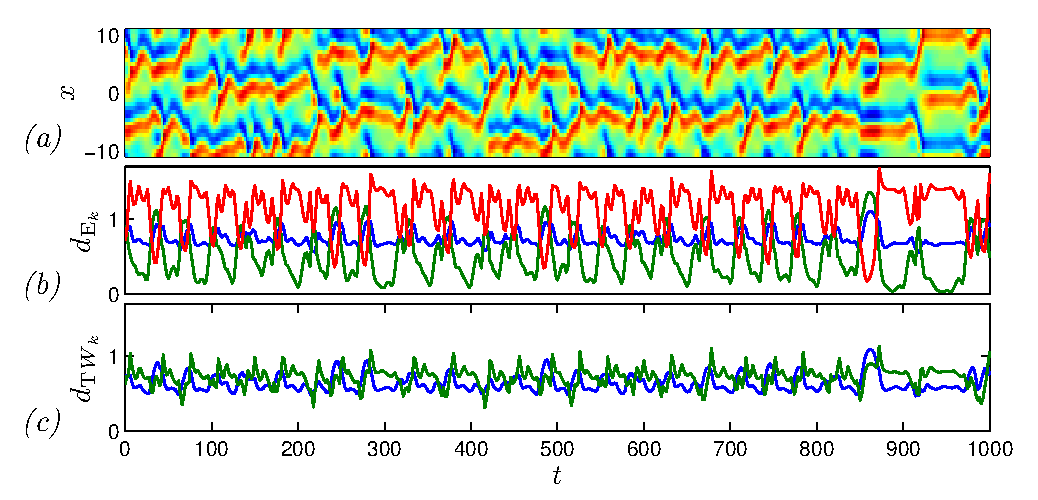
\includegraphics[width=0.9\textwidth, clip=true]{ks_prox_eq_tw}
\end{center}
\caption{\color{blue}
Proximity of a typical chaotic orbit of the \KSe with $L =
22$ to \eqva\ and \reqva. (a) chaotic orbit (same as in
refFig~{f:ks\_L22}); ~(b) distances of the chaotic orbit to
\eqva\ $\EQV{1}$, $\EQV{2}$, and $\EQV{3}$, are shown by
blue, green, and red lines, respectively. The distances are
measured according to \refeq{eq:proxeq}; ~(c) distances of
the chaotic orbit to \reqva\ TW$_{\pm 1}$ and TW$_{\pm 2}$,
are shown by blue, and green lines, respectively. The
distances are measured according to \refeq{eq:proxtw}.
     } \label{f:ks_prox_eq}
\end{figure}
%%%%%%%%%%%%%%%%%%%%%%%%%%%%%%%%%%%%%%%%%%%%%%%%%%%%%%%%%%%%%%%%%%

In order to illustrate the relative influence of \eqva\ and \reqva\ on the dynamics
within the KS chaotic attractor for $L = 22$, we calculated the distance of a
typical orbit, to different \eqva\ and \reqva.

The distance of a state-space point $a$ to \eqv\ $a_{\EQV{k}}$ is measured as a
Euclidean distance in Fourier space minimized with respect to the translation
of the \eqv\ by $\Shift_{\shift/L}$:
\beq
  d_{\EQV{k}} = \min_\shift \|a - \Shift_{\shift/L} a_{\EQV{k}} \|\,,\quad k = 1,2,3.
\ee{eq:proxeq}
Similarly, the distance to \reqv\ $a_{\REQV{\pm}{k}}$ is defined as follows
\beq
  d_{\REQV{k}{}} = \min_{\shift} \|a - \Shift_{\shift/L} a_{\REQV{\pm}{k}} \|\,,\quad k = 1,2,
\ee{eq:proxtw}
where we consider the distance to both $a_{\REQV{-}{k}}$ and $a_{\REQV{+}{k}}$, thus
minimizing both with respect to translation $\Shift_{\shift/L}$ and reflection $\Refl$.

The plot of $d_{\EQV{k}}$ in \reffig{f:ks_prox_eq}(b) show that \EQV{2} has a dominant
influence on the dynamics, \EQV{3} is influencing the dynamics more intermittently, while
\EQV{1} has little effect on the dynamics.  Similarly, as shown in \reffig{f:ks_prox_eq}(c),
the chaotic orbit does not visit the neighborhoods of \reqva , so their influence on
the chaotic dynamics is also minimal.

\subsection{Norms blog}

\begin{description}
\item[2011-11-16 Predrag] My problem is with the norm, or notion of
distance used in siminos/ksReduced. In fluid dynamics the community has
settled on
\beq
  \Norm{\ssp-\ssp'}^2  = \braket{\ssp-\ssp'}{\ssp-\ssp'} =
\frac{1}{V}
\int_\bCell \! d \bx \;
(\vec{u}-\vec{u}') \cdot (\vec{u}-\vec{u}')
\,.
\ee{innerproduct}
There is no compelling reason to use this {`energy norm'}, other than
that velocity fields is what is given in a numerical computation. What
norm one actually uses depends very much on the application. In the study
of `optimal perturbations' that move a laminar solution to a turbulent
one, both energy \citep{TeHaHe10} and dissipation \citep{LoCaCoPeGo11}
norms have been used.

If field $u(x,t)$ in \KSe\  is interpreted as
`flame-front velocity', the time-dependent $L^2$ norm
of $u$,
\beq
  \expctE= \Lint{\pSpace} V(x,t)= \Lint{\pSpace} \frac{u^2}{2}
  \,,
  \label{ksEnergy}
\eeq
has a physical interpretation\rf{ksgreene88} as the average `energy'
density of the flame front, in analogy to the mean kinetic energy
density for the Navier-Stokes.
I think for \KS\ it would be the safest to use
\beq
  \Norm{\ssp-\ssp'}^2  = \braket{\ssp-\ssp'}{\ssp-\ssp'} =
\Lint{\pSpace} ({u}-{u}')^2
\,.
\ee{KSnorm}
The virtue of energy norm is that it is representation independent. If
one goes to siminos/ksReduced/ invariant basis, the $2N-1$
$\SOn{2}$-invariant and functionally independent variables are
\bseq\label{eq:SO2cheb}
  \begin{align}
    \overline{b}_k &=
		    b_k\, \chebT_k\left(b_1/r_1\right)+
		    c_k\,\frac{c_1}{r_1} \chebU_{k-1}\left(b_1/r_1\right)\,, \label{eq:SO2cheb1}\\
    \overline{c}_k &=
		    b_k\, \frac{c_1}{r_1} \chebU_{k-1}\left(b_1/r_1\right)+
		    c_k\,\chebT_k\left(b_1/r_1\right)\,,  \label{eq:SO2cheb2}
  \end{align}
\eseq
for $k=1,\ldots N$, where $r_k\equiv\sqrt{b_i^2+c_i^2}$ and $\chebT_k,\,\chebU_k$
are Chebyshev polynomials of the first and second type, respectively.
The Chebyshev polynomials $\chebT_k,\,\chebU_k$ are degree $k$, so they tend
to significantly distort the \statesp\ layout of the attractor.

Evangelos, please confirm that you are using distance function \refeq{KSnorm},
not the norm
\beq
\Norm{u}  =   {\textstyle\frac{1}{2}} \sum_{k=0}^{\infty}
   (\overline{b}_k^2+\overline{c}_k^2)
\,,
\ee{normNotGood}



\end{description}

\section{Freeze! drop that knife, no slicing here}
\label{sect:freeze}
\renewcommand{\LieElrep}{\ensuremath{g}} % Siminos Lie group element

\begin{description}

\item[2011-11-01 Ruslan] (muttering to himself)             \toCB
I know Predrag wants to do it on a slice, but
i) I'm yet to see a sliced KS and
ii) I'm not convinced that slicing is useful in high dimensions anyway:
I can see the benefit of reducing a 3-d flow to a 2-d map, but I'm not
sure it is as beneficial to work with a 6-d map instead of an 8-d flow.

\item[2011-11-04 Predrag]              \toCB
How high does 100.000 dimensions sound to you?

i) I have said ciao to Chao, so currently no one is slated to slice
\KS.

ii) Instead, we have sliced transitionally turbulent pipe flow, and
for the first time we have \rpo s embedded in pipe turbulence. The great
advantage of the pipe flow is that it has no streamwise reflection
symmetry, so all exact solutions are relative, and there is no room for
philosophy - you either do it or do not do it. \emph{Invite Ashley Willis
for a seminar}.

iii) Every continuous symmetry must be reduced in order
to organize the flow, a local chart describing a neighborhood of a
template is a slice in group action directions, Poincar\'e section in
time evolution directions. One MUST go to Poincar\'e section to organize
the attractor by local stable-manifold road maps. In \pCf\ we have many
\po s, but together they just make a jumble in the \statesp. It's obvious
why if you just work through the 3-disk example in ChaosBook.org - only
in the Poincar\'e section is the topology of the strange attractor
cleanly laid out. (Getting this across has ballooned ChaosBook's
initial 2-chapter review of dynamics into 10 chapters and counting...)

\item[2011-11-04 Ruslan] Thank you for replying to my 'muttering', and
thanks for the suggestion: will invite Ashley over.  Indeed things are
much easier without reflections.  I agree with (iii) if a good slice can
be found, but the 'curse of dimensionality' will be hard to beat.  Your
slice quilt in \reffig{fig:Tesselate} looks good in 2-d (with 16 slices),
but in $n$-d you'll need $4^n$ slices to achieve the same resolution.

\item[2011-11-04 Predrag] Too pessimistic. If the `physical dimension' is
large, we are indeed screwed. If it is 4-8 (\KS) or 100-1000 (\pCf\ in
the minimal cell) I expect the number of qualitatively different states
to be a handful, a factor of 2-4 for each spatial direction.
%If you think
%$3D$ turbulent pipe flow is `much easier' be my guest - go do it. It will
%be news to Ashley and Marc who did not get the memo.
%
%\item[2011-11-04 Ruslan] I did not say pipe flow was easy, I was rather
%referring to something like CLE.

\item[2011-11-04 Ruslan]
But even if we only do it locally, in order to really tackle the symmetry
reduction problem in \KS, I'd suggest we try to do it not around one of
the RPOs or PPOs, but in the vicinity of the $\EQV{2} \to
\tau_{1/4}\EQV{2}$ heteroclinic cage.  We claimed in our paper that it
organizes the \KS\ flow for $L = 22$, now it would be good to put some
meat on this carcass.

\item[2011-11-04 Predrag] Agreed. We do not have enough experience with
actually picking good templates, we should try various choices. My
understanding is that a good set of templates should enumerate all topologically
distinct states of the system. For example, for a stretch \&\ fold flow
one needs two, one for `stretch' part of the unstable manifold, the other
for `stretch \&\ flip' part. The embedding dimension does not matter.
The problem is manpower.

\item[2011-11-05 Ruslan] Manpower is not a problem if we are all pulling
in the same direction.  If you agree that the case of the
$\EQV{2} \to \tau_{1/4}\EQV{2}$ heteroclinic cage is sufficiently interesting,
then we are returning back to my dilemma
I expressed in 2009-10-17 (Desymmetrization blog, section 13.9).

\item[2011-11-07 ES] My opinion on how to proceed can now be found
in siminos/ksReduced. Let's continue the discussion in siminos/blog.

\item[2011-11-04 Predrag 2 Ruslan] Something completely different. My
undergraduate Naveen is simulating the \emph{Karma model} of cardiac
activity introduced by Alain Karma (\emph{Electrical alternans and spiral
wave breakup in cardiac tissue}\rf{Karma1994}). It is a 1\dmn\ PDE on a
periodic ring, with using state variables $E$, which is the value for the
voltage in cardiac tissue, and $n$, which is the slow current gate
variable.

Can you \rpo\ fishing programs be easily altered from KS to another
1\dmn\ PDE?

\item[2011-11-05 Ruslan about Karma model]  How interesting... I know
Alain very well through his work on phase field modelling of solid-liquid
interfaces.  I had no idea that in his previous incarnation he worked in
nonlinear dynamics.  I heard of cardiac Karma model before, but I
honestly thought it was a different Karma, until you mentioned Alain.
Anyway, sure I can have a look at it, just need to be able to integrate
this PDE numerically with under about 100 ODEs.  I don't have access to
Chaos here, so it would be useful if you (or Naveen) spelled out for me
the equations, parameters, dynamics you are interested in, etc.

\item[2011-11-05 Predrag] Karma 1994 paper:
\HREF{http://chaosbook.org/library/Karma1994.pdf}
{click here}. You will need to type \texttt{student} and then \texttt{Lautrup} .

\item[2011-11-15 Predrag] (Less minor:) sooner or later you have to bite
a bullet and start looking at the periodic points and their unstable
manifolds in sets of Poincar\'e sections defined at well chosen template
points. \refFig{fig:ks22shad} quickly becomes a meaningless jumble (that
is what Gibson does with our \pCf\ \po s; nothing can be
understood this way). I'm worried that siminos/ksReduced
approach will not work for high-dimensional flows (it is no different
from using low Fourier modes to capture highly turbulent states), but
I'll shut up - if you make it work for \KS, I'll be impressed.

\begin{figure}[ht]
  \begin{center}
    (a)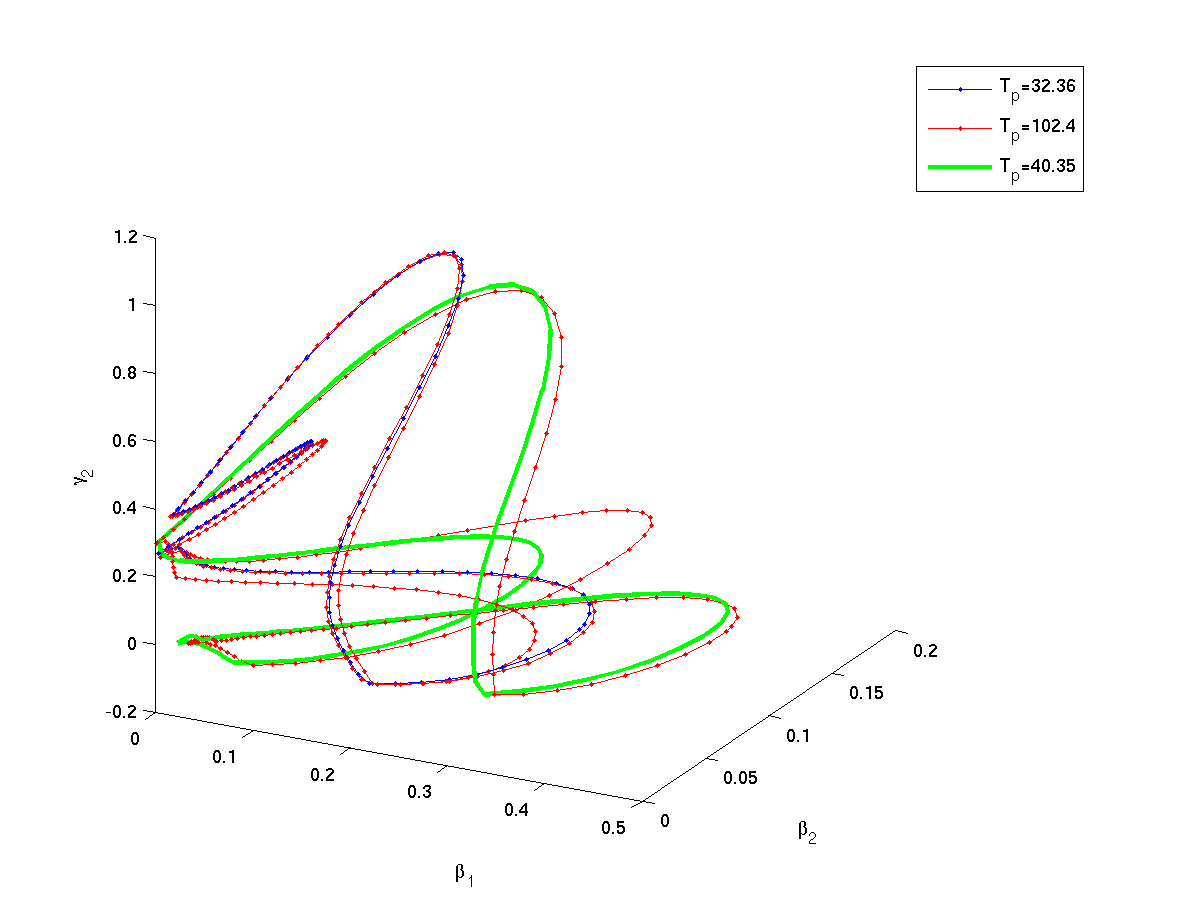
\includegraphics[width=0.45\textwidth]{ks22ppoT10235shad.png}~
    (b)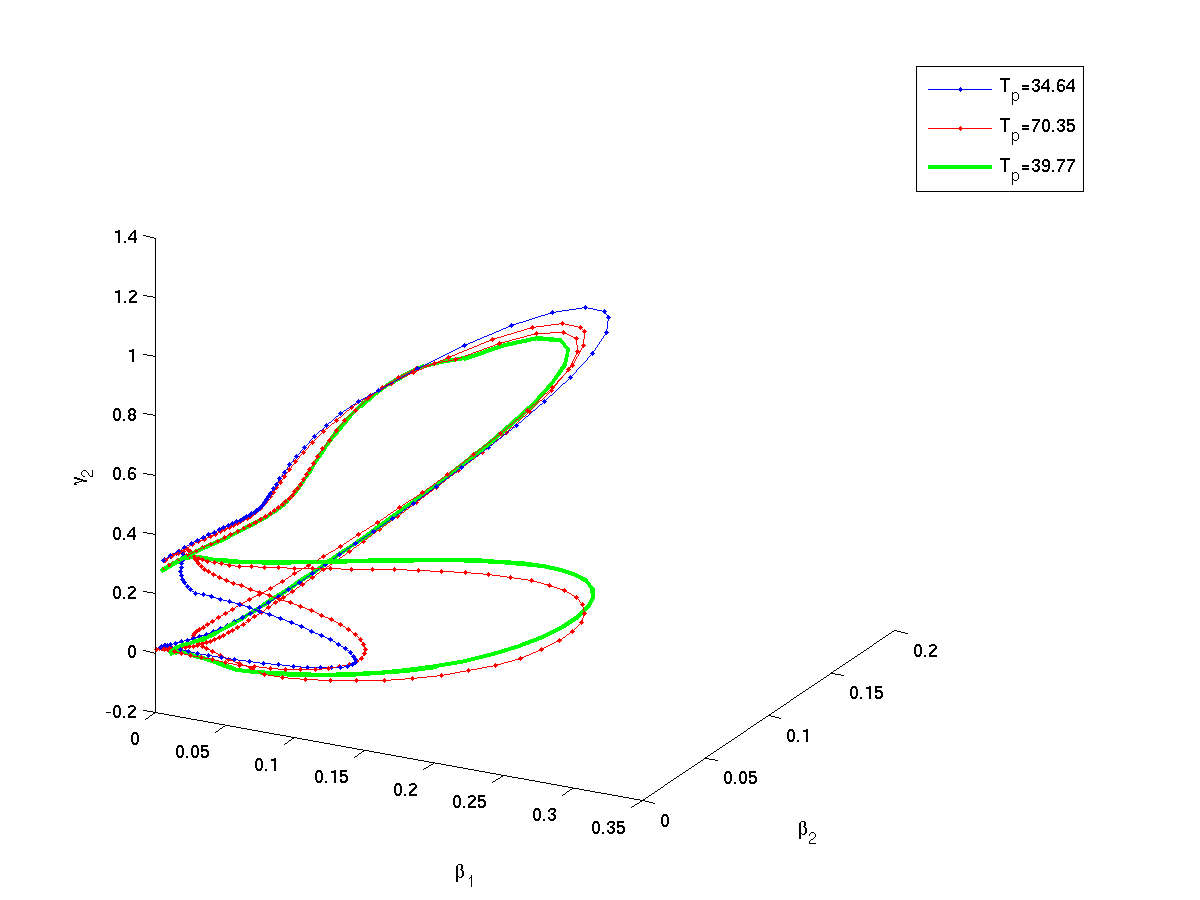
\includegraphics[width=0.45\textwidth]{ks22ppoT7035shad.png}\\
    (c)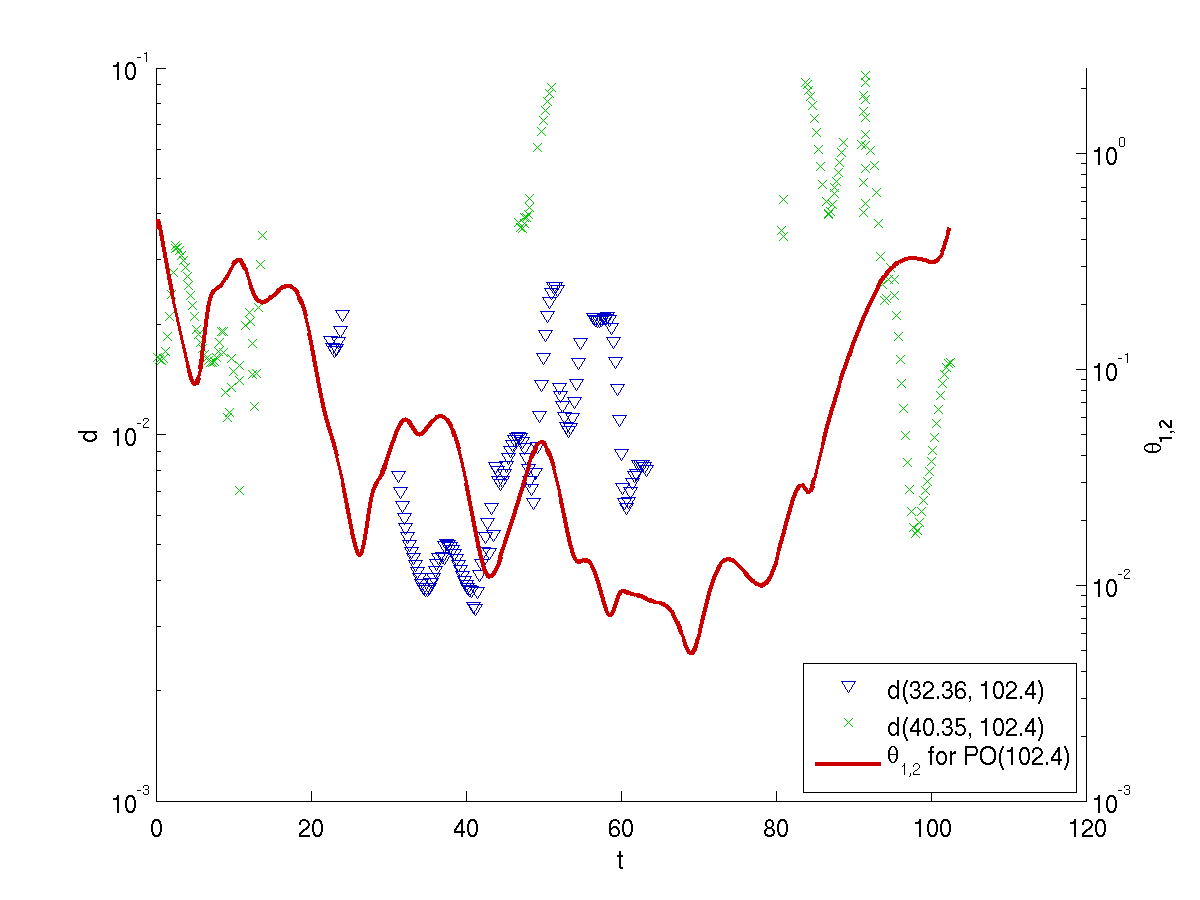
\includegraphics[width=0.45\textwidth]{ks22ppoT10235angl_dist.png}~
    (d)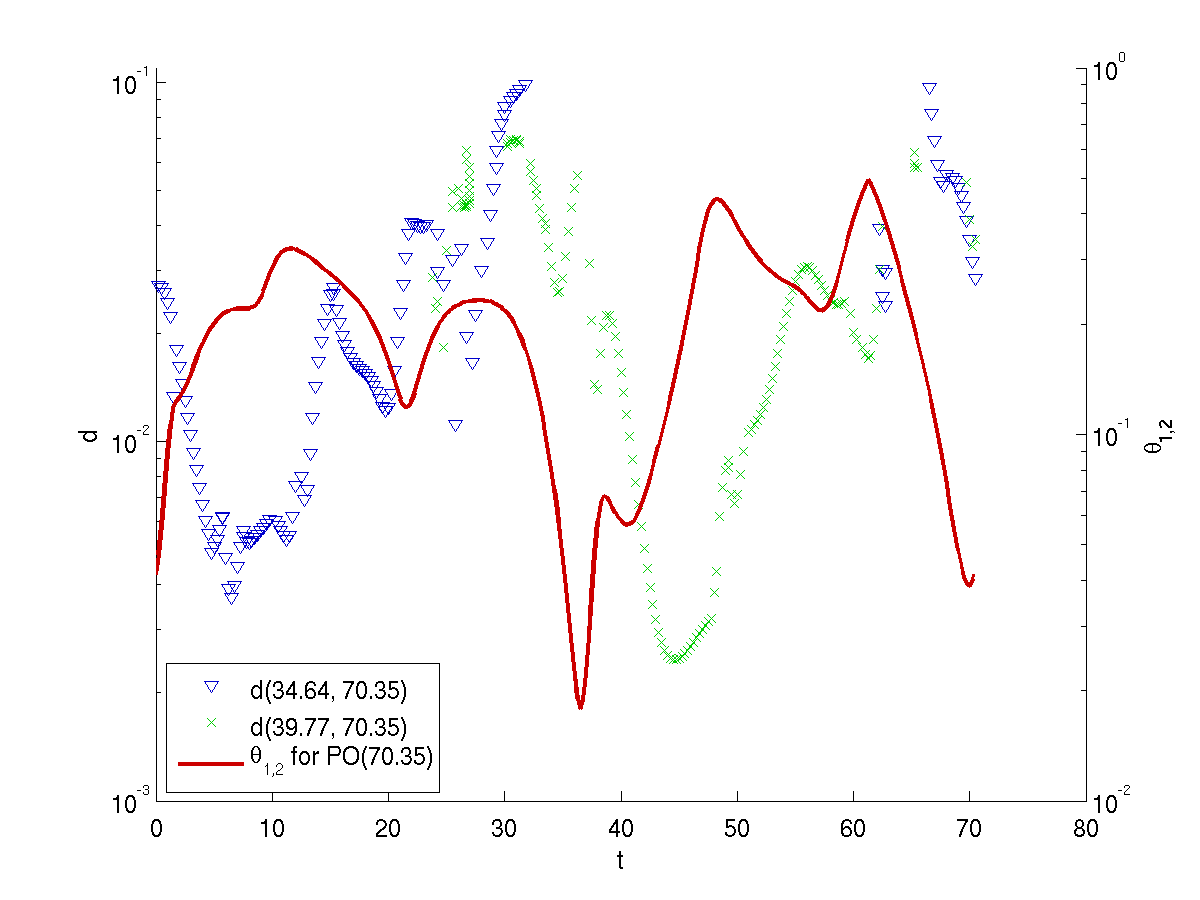
\includegraphics[width=0.45\textwidth]{ks22ppoT7035angl_dist.png}
  \end{center}
  \caption{Shadowing of periodic orbits. (a) Hyperbolic pre-periodic orbits
    \PO{32.36} and \PO{40.35} shadow \PO{102.4} which appears to be close
    to non-hyperbolicity. Note that \PO{102.4} traces \PO{32.36} twice.
    (b) \PO{70.35}, is shadowed by \RPO{34.64} and \RPO{39.77}.
    (c) Angle of first two Floquet eigenvectors along \PO{102.4} (red, solid line) and
    closest distance from \PO{102.4} of points on \PO{32.36} (blue triangles) and \PO{40.35}
    (green crosses). (d) Angle of first two Floquet eigenvectors along \PO{70.45} (red, solid line) and
    closest distance from \RPO{70.45} of points on \PO{34.64} (blue triangles) and \RPO{39.77}
    (green crosses).
    }
  \label{fig:ks22shad}
\end{figure}


\item[2011-11-16 Evangelos] The scope of siminos/ksReduced would be to
demonstrate symmetry reduction, not to reduce \KS\ flow to return maps.
The latter would be left to some subsequent paper and indeed someone will have
to bite a bullet and do what you suggest (maybe this will be me anyway).

`` It is no different from using low Fourier modes to capture
highly turbulent states.'' I disagree. \refFig{fig:ks22shad}(a)
and (b) indeed focus on low Fourier modes but they are just a visual aid,
not really needed here. On the other hand distance in
\reffig{fig:ks22shad}\,(c) and (d) is computed in invariant variables using
\emph{all} Fourier modes (\ie\ as many as you need for a well resolved
simulation). For the Lyapunov project \reffig{fig:ks22shad}(c) and (d)
and \reftab{tab:ks22shad} are, I think, good starting points to formulate
a conjecture.

\item[2011-11-16 Evangelos]
Ideally, siminos/ksReduced would include:
\begin{itemize}
 \item some visualizations of unstable manifolds of \eqva\ and \reqva\
	in invariant variables, projected on local coordinate systems
	given by the least stable eigenvectors as in our
	SIADS paper \refref{SCD07},
 \item some visualizations illustrating how (relative) periodic orbits are
	organized by such unstable manifolds (corroborated by measuring distance
	of points on the cycles from points on the unstable manifolds),
 \item some rudimentary organization of short cycles into families using
	their mutual distance as criterion.
\end{itemize}

At this stage I don't see anything wrong with publishing a paper that does
not tell the whole \KS\ story (even achieving 2 out of 3 goals above is a lot
of work and even writing down the symmetry invariant variables required a lot
of thinking).

\item[2011-11-16 Predrag] You are right, a step at a time. Let's go for
it. As for the massaged invariant variables of siminos/ksReduced, all is
fair in war and love.



\end{description}

\renewcommand{\ssp}{a}
